% !TeX encoding = UTF-8
% !TeX program = pdflatex
% !TeX spellcheck = it_IT

\documentclass[binding=0.6cm,TFA]{sapthesis}

\usepackage{microtype}
\usepackage[italian]{babel}
\usepackage[utf8]{inputenx}

\usepackage{hyperref}
\hypersetup{pdftitle={Analisi delle problematiche di sicurezza del protocollo MQTT},pdfauthor={Edoardo Di Paolo}}

% Remove in a normal thesis
\usepackage{lipsum}
\usepackage{curve2e}
\usepackage{setspace}
\onehalfspacing

%code related
\usepackage{pythonhighlight}


\definecolor{gray}{gray}{0.4}
\newcommand{\bs}{\textbackslash}

% Commands for the titlepage
\title{Analisi delle problematiche di sicurezza del protocollo MQTT}
\author{Edoardo Di Paolo}
\IDnumber{1728334}
\course{Corso di Laurea in Informatica}
\courseorganizer{Facoltà di Ingegneria dell'informazione, informatica e statistica}
\AcademicYear{2019/2020}
\copyyear{2020}
\advisor{Prof. Angelo Spognardi}
%\advisor{Dr. Nome Cognome}
%\coadvisor{Dr. Nome Cognome}
\authoremail{dipaolo.1728334@studenti.uniroma1.it}

%\examdate{ }
%\examiner{ }
%\examiner{Prof. Nome Cognome}
%\examiner{Dr. Nome Cognome}
%\versiondate{\today}




\begin{document}

\frontmatter

\maketitle

\dedication{Alla mia famiglia.\\}

%\begin{acknowledgments}
%Ringraziamenti
%\end{acknowledgments}


%\begin{abstract}
%Introduzione
%\end{abstract}


\tableofcontents

% Do not use the starred version of the chapter command!



\mainmatter
\chapter{Introduzione}

\begin{large}
Negli ultimi decenni il numero di dispositivi collegati ad Internet è cresciuto rapidamente; non ci sono più, infatti, solo computer o cellulari in rete ma anche elettrodomestici, macchine industriali e strumenti medici, tutti dispositivi che fino a qualche anno fa erano offline. Tutto ciò fa riferimento all'IoT, l'\textit{Internet of Things}. \\
Parallelamente allo sviluppo di queste nuove tecnologie, sono stati studiati nuovi protocolli per far si che i dispositivi possano essere utilizzati in maniera efficiente; ci sono, ad esempio, alcuni sensori i quali permettono di misurare temperatura ed umidità di una stanza funzionando attraverso l'uso di una semplice pila; è necessario, quindi, andare a ridurre il costo energetico della connessione così da aumentare la durata di utilizzo del dispositivo. \\
Alcuni esempi di protocolli possono essere: MQTT, CoAP, AMQP e WebSocket che hanno la possibilità di essere integrati con TLS (\textit{Transport Layer Security}) così da poter garantire una maggiore sicurezza nello scambio dei dati anche se, in realtà, ciò potrebbe andare a gravare sui consumi del dispositivo poiché dovrebbero essere effettuati più calcoli affinché avvenga il trasporto dei dati. Inoltre, con l'aumento di questi nuovi dispositivi sono aumentate anche le possibili minacce relative all'IoT. Un esempio è il malware Mirai \cite{wiki:Mirai} che, nel 2016, ha infettato milioni di dispositivi rendendoli parte di una botnet che, successivamente, ha attaccato attraverso un DDoS il fornitore di servizi DNS Dyn così da rendere inaccessibili milioni di siti web. A causa, anche, di questa tipologia d'attacco, sempre più comune, i protocolli sviluppati devono presentarsi sicuri e robusti.\\

Negli ultimi anni l'utilizzo del protocollo MQTT è sicuramente cresciuto di gran misura.
\begin{figure}[h]
\centering
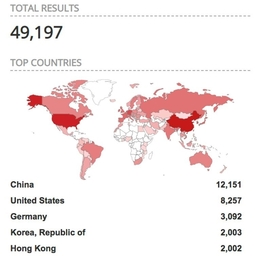
\includegraphics[scale=0.8]{images/mqtt-2018numbers.jpg}
\caption{Numero dispositivi MQTT 2018.}
\label{fig:mqtt2018}
\end{figure}

La \autoref{fig:mqtt2018} rappresenta il numero di dispositivi che una ricerca della parola "MQTT" produceva nel 2018 sul sito Shodan \cite{articleAvast}.
Se effettuiamo la stessa ricerca adesso, ne abbiamo un numero maggiore, come dimostra la figura sottostante.

\begin{figure}[h]
\centering
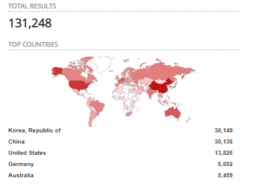
\includegraphics[scale=0.8]{images/mqtt-2020numbers.png}
\caption{Numero dispositivi MQTT 2020, statistiche di Shodan \cite{shodan}.}
\label{fig:mqtt2020}
\end{figure}

La maggior parte di questi dispositivi girano sulla porta standard di MQTT, la 1883 e molti di questi non richiedono alcuna autenticazione per poter connettersi. Effettuando una ricerca ancora più specifica attraverso la stringa "\textit{port:1883}", abbiamo di nuovo più risultati come si vede dalla \autoref{fig:mqttport2020}.\\

\begin{figure}[h]
\centering
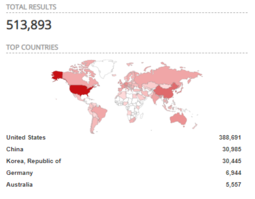
\includegraphics[scale=0.8]{images/mqtt-2020port.png}
\caption{Numero dispositivi MQTT 2020, port:1883.}
\label{fig:mqttport2020}
\end{figure}

In questa relazione viene descritto lo studio effettuato su uno dei maggiori protocolli nell'IoT: MQTT. Nello specifico durante l'attività di tirocinio siamo andati alla ricerca di possibili anomalie e/o violazioni del protocollo da parte dei broker server i quali dovrebbero rispettare ogni standard definito per MQTT. \\

Nel \textbf{Capitolo 2} è analizzato il protocollo nel dettaglio assieme alle sue principali caratteristiche e funzionalità. \\

Nel \textbf{Capitolo 3} viene analizzata la libreria che è stata scritta ai fini del tirocinio. In questo capitolo sono anche descritti i differenti broker e il dispositivo fisico sui quali sono stati effettuati i test. Inoltre vengono riportati i risultati di alcuni esperimenti. \\

Nel \textbf{Capitolo 4} sono riportate le conclusioni del lavoro svolto durante il tirocinio.

\end{large}


\chapter{MQTT}

\begin{large}

\section{Descrizione del protocollo}

MQTT, acronimo di \textit{Message Queuing Telemetry Transport}, è un protocollo di tipo \textit{publish-subscribe} che permette il trasporto di messaggi tra diversi dispositivi tramite TCP/IP. Il protocollo è molto utilizzato in ambito IoT per la sua semplicità e anche per la banda la cui richiesta è davvero bassa. \\

MQTT presenta un modello di architettura differente, ad esempio, dal tipico client/server del protocollo HTTP; infatti adotta il meccanisco \textit{publish-subscribe} (pub/sub) attraverso l'utilizzo di un \textit{broker}. Il funzionamento del modello pub/sub avviene attraverso la pubblicazione e la sottoscrizione da parte del client a diversi topic, che possono essere paragonati a dei canali di comunicazione. In MQTT il publisher e il subscriber non comunicano mai direttamente e non sono neppure consapevoli della presenza dell'uno e dell'altro: il collegamento è gestito dal broker il cui compito è quello di filtrare i messaggi che riceve e distribuirli ai vari subscribers. 
In questo capitolo sono analizzate le principali caratteristiche che il protocollo MQTT mette a disposizione.
%shodan stats (?)

\subsection{Topic}
Nel protocollo MQTT un topic non è altro che una stringa codificata in UTF-8 che il broker utilizza per filtrare i messaggi da inviare successivamente ad ogni client sottoscritto a quel topic. I topic sono case-sensitive, pertanto bisogna prestare attenzione alle lettere maiuscole o minuscole e alla lunghezza minima di un carattere. Inoltre, MQTT mette a disposizione del client dei \textit{wildcard} che permettono di connettersi simultaneamente a più topic; uno è rappresentato dal simbolo +, mentre l'altro dal simbolo \#. Il primo è chiamato \textit{single-level} wildcard, il secondo \textit{multi-level} wildcard. Ci sono dei topic ai quali non si può pubblicare alcun messaggio; sono riservati allo stato del sistema e sono cominciano per \$SYS/. \\
Alcuni esempi di topic validi possono essere i seguenti: 
\begin{enumerate}
\item \textit{casa/luci/sala} - topic specifico per le luci della sala;
\item \textit{casa/+/sala} - include tutti i topic dei dispositivi che fanno riferimento alla sala (luci comprese);
\item \textit{casa/\#} - include tutti i topic che fanno riferimento alla casa.
\end{enumerate}


\subsection{Connessione al broker}
Come scritto nell'introduzione di questo capitolo, la connessione avviene solamente fra client e broker. Per client intendiamo un qualsiasi dispositivo il quale permette di gestire una connessione ad un broker che si comporta similmente ad un server. 

\begin{figure}[h]
\centering

\includegraphics[width=0.7\textwidth]{images/connect-connack.png}
\caption{Flusso connessione al broker MQTT.}
\label{fig:connect-connack}
\end{figure}

Come si può vedere dalla \autoref{fig:connect-connack}, la connessione avviene tramite lo scambio di due pacchetti: \textit{connect}, inviato dal client al broker e \textit{connack} inviato dal broker al client. Il pacchetto connect contiene i seguenti parametri:
\begin{table}[h]
\caption{Parametri pacchetto connect.}
\label{tab:connect}
\begin{tabular}{lp{0.8\textwidth}}
\toprule
\textbf{Parametro} & \textbf{Descrizione} \\
\midrule
\textit{clientId} & rappresenta l'identificativo del client che chiede di connettersi \\
\textit{cleanSession} & valore booleano il quale specifica se la connessione è persistente o meno \\
\textit{username} & rappresenta l'username necessario affinché avvenga la connessione \\
\textit{password} & la password associata all'username \\
\textit{willRetain} & viene letto solo se \textit{willFlag} è true \\
\textit{willQos} & viene letto solo se \textit{willFlag} è true \\
\textit{willFlag} & permette di notificare un messaggio specificato dal client nel payload in caso di disconnessione anomala \\
\textit{keepAlive} & rappresenta in secondi l'intervallo massimo in cui broker e client possono non inviarsi messaggi \\
\bottomrule
\end{tabular}
\end{table}

Il pacchetto connack, invece, è così strutturato: \\
\begin{table}[h]
\caption{Parametri pacchetto connack.}
\label{tab:connack}
\begin{tabular}{lp{0.8\textwidth}}
\toprule
\textbf{Parametro} & \textbf{Descrizione} \\
\midrule
\textit{sessionPresent} & flag riferita al cleanSession del pacchetto connect \\
\textit{returnCode} & stato della connessione \\
\bottomrule
\end{tabular}
\end{table}

Per quanto riguarda il \textit{returnCode} descritto nella \autoref{tab:connack}, questo è un valore che va da 0 a 5:
\begin{itemize}
\item 0: connessione accettata;
\item 1: connessione rifiutata, versione del protocollo non valida;
\item 2: connessione rifiutata, clientId non valido;
\item 3: connessione rifiutata, server non disponibile;
\item 4: connessione rifiutata, username o password errati;
\item 5: connessione rifiutata, non autorizzati.
\end{itemize}

\subsection{Sottoscrizione e pubblicazione}
Come scritto più volte, MQTT è un protocollo che adotta un meccanismo chiamato \textit{publisher/subscribe}; perciò le due azioni fondamentali che un client può compiere sono \textit{publish} e \textit{subscribe}.
\subsubsection{Subscribe}
L'azione subscribe permette al client di sottoscriversi a un determinato topic passato nel pacchetto.

\begin{figure}[h]
\centering
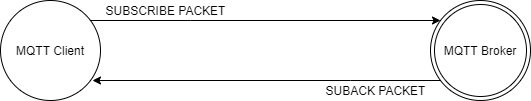
\includegraphics[width=0.7\textwidth]{images/subscribe-suback.png}
\caption{Flusso subscription ad un topic in MQTT.}
\label{fig:subscribe-suback}
\end{figure}

Come si nota dalla \autoref{fig:subscribe-suback}, la sottoscrizione avviene semplicemente con lo scambio di due pacchetti: \textit{subscribe}, dal client al broker, e \textit{suback}, dal broker al client. Il primo pacchetto rappresenta la richiesta di sottoscrizione ad un determinato topic, il secondo invece conferma la sottoscrizione a quel topic. \\
I parametri del subscribe packet sono i seguenti:

\begin{table}[h]
\caption{Parametri pacchetto subscribe.}
\label{tab:subscribe}
\begin{tabular}{lp{0.8\textwidth}}
\toprule
\textbf{Parametro} & \textbf{Descrizione} \\
\midrule
\textit{packetId} & l'identificatore del pacchetto \\
\textit{payload} & una lista di QoS e topic a cui sottoscriversi \\
\bottomrule
\end{tabular}
\end{table}
Il pacchetto suback, invece, è così strutturato:
\begin{table}[h]
\caption{Parametri pacchetto suback.}
\label{tab:suback}
\begin{tabular}{lp{0.8\textwidth}}
\toprule
\textbf{Parametro} & \textbf{Descrizione} \\
\midrule
\textit{packetId} & l'identificatore del pacchetto a cui rispondere \\
\textit{returnCode} & lista di \textit{returnCode} che rappresentano lo stato della sottoscrizione \\
\bottomrule
\end{tabular}
\end{table}

Anche in questo caso il \textit{returnCode} può assumere diversi valori, riassunti in questa lista:
\begin{enumerate}
\item 0: successo, massimo QoS 0;
\item 1: successo, massimo QoS 1;
\item 2: successo, massimo QoS 2;
\item 128: sottoscrizione fallita.
\end{enumerate}

All'azione di sottoscrizione corrisponde anche un'azione di disiscrizione dal topic che avviene attraverso il pacchetto \textit{unsubscribe}. Quest'ultimo è così strutturato:
\begin{table}[h]
\caption{Parametri pacchetto unsubscribe.}
\label{tab:unsubscribe}
\begin{tabular}{lp{0.8\textwidth}}
\toprule
\textbf{Parametro} & \textbf{Descrizione} \\
\midrule
\textit{packetId} & l'identificatore del pacchetto a cui rispondere \\
\textit{topics} & lista di topic da cui disiscriversi \\
\bottomrule
\end{tabular}
\end{table}

\subsubsection{Publish}
La pubblicazione di un messaggio in MQTT è più complicata rispetto alla fase di sottoscrizione al topic. Prima di tutto, bisogna introdurre il concetto di QoS, \textit{Quality of Service}. Il QoS è paragonabile ad un contratto che viene stipulato tra client e broker; esistono tre diversi livelli: QoS 0, QoS 1, QoS 2.


Nel Quality of Service di livello 0 il payload del pacchetto viene pubblicato immediatamente. In questo caso non c'è garanzia sull'effettiva pubblicazione del messaggio.
\begin{figure}[h]
\centering
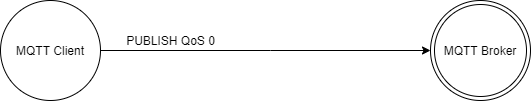
\includegraphics[width=0.7\textwidth]{images/publish-qos0.png}
\caption{Flusso publish con QoS 0.}
\label{fig:qos-0pub}
\end{figure}

Nel caso del Quality of Service di livello 1 viene garantita la pubblicazione ad almeno un destinatario.
\begin{figure}[h]
\centering
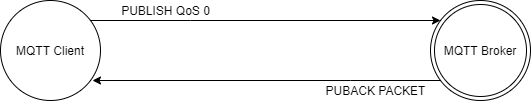
\includegraphics[width=0.7\textwidth]{images/publish-qos1.png}
\caption{Flusso publish con QoS 1.}
\label{fig:qos-1pub}
\end{figure}

Come si vede dalla \autoref{fig:qos-1pub}, il client riceve dal broker il pacchetto \textit{puback} solo dopo aver pubblicato il pacchetto publish. 
Il pacchetto puback è così strutturato:
\begin{table}[h]
\caption{Parametri pacchetto puback.}
\label{tab:puback}
\begin{tabular}{lp{0.8\textwidth}}
\toprule
\textbf{Parametro} & \textbf{Descrizione} \\
\midrule
\textit{packetId} & l'identificatore del pacchetto publish \\
\bottomrule
\end{tabular}
\end{table}

Questo meccanismo permette al client di inviare nuovamente il pacchetto publish nel caso in cui, dopo un certo intervallo di tempo, non abbia ancora ricevuto il puback dal broker; in questo caso, nel pacchetto publish, il campo \textit{dup} sarà impostato come true. Inoltre, il client mantiene in memoria il pacchetto publish finché non riceve il puback.

Infine abbiamo il QoS di livello 2 il quale dà maggiore affidabilità ma è più lento rispetto ai precedenti livelli.

\begin{figure}[h]
\centering
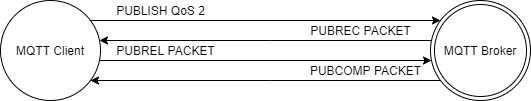
\includegraphics[width=0.7\textwidth]{images/publish-qos2.png}
\caption{Flusso publish con QoS 2.}
\label{fig:qos-2pub}
\end{figure}

Come si vede dalla \autoref{fig:qos-2pub} abbiamo più messaggi scambiati fra client e broker. Questo meccanismo assicura che il messaggio sia ricevuto solamente una volta dai destinatari; il livello 2, perciò, dà un maggiore livello di sicurezza al client.
Nel caso in cui il pacchetto vada perso, dopo un certo intervallo di tempo il client trasmetterà nuovamente il pacchetto e resterà in attesa della risposta da parte del broker. \\
La struttura dei pacchetti è la stessa che si può vedere nella \autoref{tab:puback}. \\

Dato che sono stati analizzati i differenti QoS, ora si può analizzare nel dettaglio il publish, il pacchetto più complicato del protocollo.
Il pacchetto ha i seguenti parametri:
\begin{table}[h]
\caption{Parametri pacchetto publish.}
\label{tab:publish}
\begin{tabular}{lp{0.8\textwidth}}
\toprule
\textbf{Parametro} & \textbf{Descrizione} \\
\midrule
\textit{packetId} & l'identificatore del pacchetto \\
\textit{topic} & il topic a cui si vuole pubblicare il messaggio \\
\textit{qos} & il Quality of Service del pacchetto \\
\textit{retainFlag} & booleana per il \textit{retained} \\
\textit{payload} & il contenuto del messaggio \\
\textit{dup} & booleana che indica se il messaggio è un duplicato \\
\bottomrule
\end{tabular}
\end{table}

Dopo aver ricevuto il pacchetto il broker processa il messaggio in base al QoS e lo invia a tutti i client sottoscritti al topic.

\begin{figure}[h]
\centering
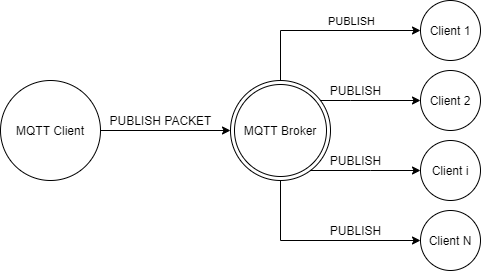
\includegraphics[width=0.7\textwidth]{images/publish-flow-example.png}
\caption{Esempio di pubblicazione di un pacchetto.}
\label{fig:publish-flow-example}
\end{figure}

\subsection{Altre caratteristiche}
\subsubsection{Retained message}
Un \textit{retained message} è semplicemente un pacchetto che ha impostato il valore true della \textit{retainFlag}. Di solito il broker una volta che riceve un messaggio da pubblicare su un topic, in cui nessun client è iscritto, lo scarta; questo avviene quando il retain è \textit{false}. Nel caso di un \textit{retained message} il broker salva in memoria il pacchetto che ha ricevuto per poi pubblicarlo una volta che un client si sottoscrive al topic.

\subsubsection{Last and will testament}
Questo meccanismo, indicato anche con \textit{LWT}, ci permette di gestire meglio le disconnessioni improvvise da parte di un client. Quando il dispositivo si connette al broker, nel pacchetto connect (\autoref{tab:connect}), viene specificato il payload nel caso in cui avvenga una disconnessione imprevista; questo payload viene salvato dal broker il quale lo utilizzerà in caso di imprevisto.

\subsubsection{Clean session o persisted session}
Questa funzionalità viene specificata dal client nel momento della connessione; infatti nel pacchetto \textit{connect} (\autoref{tab:connect}) viene specificata una variabile \textit{cleanSession}. Nel caso di una persisted session il client riceverà dal broker tutti i messaggi pubblicati sui topic a cui si era sottoscritto che sono stati inviati mentre era offline.


\subsubsection{MQTT 5}
Questa versione del protocollo è stata rilasciata nel 2018 e non è ancora utilizzata da tutti i dispositivi. Rispetto alla precedente versione, sono stati aggiunti i \textit{reason codes} i quali riportano il tipo di errore relativo al protocollo che è avvenuto. La \textit{clean session} non è più presente e al suo posto c'è la flag \textit{clean start}. È stato aggiunto anche un nuovo pacchetto, l'\textit{AUTH} packet, utilizzato ad esempio per le autenticazioni \textit{OAuth}. Il pacchetto \textit{disconnect} in MQTT 5 è bi-direzionale: il broker invia un pacchetto di tipo \textit{disconnect} prima di chiudere la connessione; in questo modo il client può intercettare il motivo della disconnessione ed agire di conseguenza.

\end{large}

\chapter{Implementazione ed esperimenti}
\begin{large}
Per ricercare possibili anomalie prodotte dalle librerie broker MQTT, vi è stata la necessità di implementare una libreria client la quale potesse permettere di gestire a basso livello i pacchetti e il loro flusso; infatti le librerie come \textit{paho} per python e \textit{mqtt.js} per nodejs non permettono di lavorare direttamente con i vari pacchetti.

\section{Implementazione del protocollo}
L'implementazione del protocollo è stata scritta in python e utilizza la libreria \textit{twisted} \cite{wiki:Twisted}. 
Sono stati implementati tutti i pacchetti che MQTT mette a disposizione, inclusi tutti i livelli QoS. \\
Un esempio di pacchetto costruito è quello publish; nella \autoref{tab:publish} possiamo vedere il \textit{fixed header} del pacchetto.

\begin{table}[h]
\caption{Fixed header publish packet.}
\label{tab:publishbytes}
\centering
\begin{tabular}{|l|c|c|c|c|c|c|c|c|}
\hline
\textbf{bit}     & 7 & 6 & 5 & 4 & 3   & 2 & 1 & 0       \\
\hline
\textbf{byte 1}  & \multicolumn{4}{|c|}{Packet} & Dup & \multicolumn{2}{|c|}{QoS level} & Retain  \\
\hline
        & 0 & 0 & 1 & 1 & x   & \multicolumn{2}{|c|}{x} & x \\
\hline
\textbf{byte 2}~ & \multicolumn{8}{|c|}{Remaining Length}                                                       \\
\hline
\end{tabular}
\end{table}

Oltre a questo header, abbiamo il \textit{variable header} che contiene il nome del topic a cui si sta pubblicando e l'id del pacchetto. Infine c'è campo per il \textit{payload}, ovvero il contenuto del messaggio da pubblicare.
\newpage

Il codice python per la gestione di questo pacchetto è il seguente:

\begin{python}
def publish(self, topic, message, dup=False, qos=0, retain=False, messageId=None):
    header = bytearray()
    varHeader = bytearray()
    payload = bytearray()
    
    header.append(0x03 << 4 | dup << 3 | qos << 1 | retain)
    varHeader.extend(_encodeString(topic.encode("utf-8")))
    
    if qos > 0:
    	if messageId is None:
    		varHeader.extend(_encodeValue(random.randint(1, 65535)))
    	else:
    		varHeader.extend(_encodeValue(messageId))
    
    payload.extend(_encodeString(message.encode("utf-8")))
    header.extend(_encodeLength(len(varHeader) + len(payload)))
    
    self.transport.write(header)
    self.transport.write(varHeader)
    self.transport.write(payload)
\end{python}

Come si può vedere, il codice rispecchia la costruzione del pacchetto così definito nell'OASIS standard \cite{oasis:publish}. Innanzitutto vengono inizializzati i tre differenti campi: header (fixed header), varHeader (variable header) e infine payload. Si può far caso a come il messageId, che è l'identificatore del pacchetto, venga utilizzato solamente nel caso in cui il QoS sia diverso da 0 questo poiché dopo il publish dovrebbe esserci un ulteriore scambio di pacchetti tra broker e client che coinvolge l'id del pacchetto. \\
Infine viene aggiunto il payload, codificato in utf-8 e viene esteso il fixed header aggiungendo la lunghezza totale tra varHeader e payload. Il trasporto vero e proprio del pacchetto dal client al broker, invece, è gestito grazie alla libreria twisted attraverso il metodo \textit{write}. \\

In maniera del tutto analoga sono stati implementati tutti gli altri pacchetti. Attraverso questa libreria client si ha accesso alla costruzione del pacchetto, cosa non possibile nelle librerie come paho; ciò ha permesso di creare dei test particolari che hanno dato risultati differenti in base al broker utilizzato. \\

Per facilitare l'esecuzione dei test da eseguire, si è creato il programma in modo che potesse prendere dei file \textit{json} i quali contenevano il flusso che la libreria doveva seguire. Questo ha permesso di poter studiare in maniera più dettagliata i diversi comportamenti da parte dei server. \\
Un esempio di test è il seguente:
\begin{python}
[   
    {
       "type": "subscribe",
       "params": {
           "topic": "test/topic"
       }     
    },

    {
        "type": "publish",
        "params": {
            "topic": "test/topic",
            "message": "pacchetto \#1",
            "qos": 0,
            "dup": false,
            "retain": false,
            "packetId": 1
        }
    }
]
\end{python}
In questo caso la libreria client gestiva due pacchetti: il primo di tipo subscribe al topic \textit{test/topic}, il secondo, invece, di tipo publish al topic \textit{test/topic} con QoS 0 e packet id 1. Ovviamente prima veniva inviato il pacchetto di tipo subscribe e solo successivamente quello di tipo publish.

\section{I broker studiati}
Sono stati presi come caso di studio differenti broker, che saranno introdotti molto brevemente in questa sezione. Ricapitolando, il broker ha la funzionalità di filtrare i messaggi che riceve dai differenti client e successivamente inviarli ai destinatari.

\subsection{Mosquitto}
Mosquitto \cite{Light2017} è uno fra i broker più famosi ed utilizzati per quanto riguarda MQTT. È leggero, open source e si adatta molto bene sia con dispositivi di poco consumo che con normali server. Supporta tutte le versioni del protocollo.

\subsection{EMQ X}
Anche EMQ X è un broker molto utilizzato. È scritto in \textit{Erlang} ed è open source; permette di gestire milioni di connessioni simultanee anche con un unico server. Oltre a supportare MQTT, supporta anche CoAP, MQTT-SN (\textit{MQTT for Sensors Networks}) e LwM2M.

\subsection{HiveMQ Community Edition}
\textit{HiveMQ Community Edition} è un altro broker scritto in Java ed open source.
Supporta MQTT a partire dalla versione 3.x fino all'ultima rilasciata che è MQTT 5. È molto utilizzato anche nei sistemi di automazione e in macchinari industriali che necessitano di un sistema real-time.

\subsection{Moquette}
Moquette \cite{Moquette} è un broker meno conosciuto scritto in java e open source. Supporta tutti i livelli di QoS e tutte le versioni del protocollo.

\subsection{Aedes}
Aedes \cite{Aedes} è un broker non troppo conosciuto scritto in NodeJS. Non supporta l'ultima versione di MQTT, ma è pienamente compatibile con la versione 3.1 e la 3.1.1. Ha molte librerie con le quali può essere integrato.

\section{Esperimenti effetuati}
La tecnica utilizzata per eseguire i test sulle librerie broker è stata simile al \textit{fuzzing}. Di per sé il fuzzing consiste in un'automazione dei test, i quali forniscono al SUT (\textit{software under test}) dati non validi o input inaspettati. Così facendo si può vedere il comportamento del software e si possono analizzare eventuali crash, buffer overflows e memory leaks. \\

I test che sono stati effettuati sulle librerie consistevano in file \textit{json} che vengono passati come input alla libreria client. In queta sezione sono riportati i file di alcuni test e i risultati prodotti che possono rappresentare un'anomalia di gestione da parte del broker.
Alcuni test effettuati sono stati creati prendendo spunto da \cite{articleTestsMQTT} e i risultati ottenuti sono del tutto simili a quelli descritti nell'articolo.
\newpage

\subsection{Publish QoS 2 e 1}
\label{chap:publishqos2e1}

\begin{python}
[    
    {
       "type": "subscribe",
       "params": {
           "topic": "test/topic"
       }     
    },
    {
        "type": "publish",
        "params": {
            "topic": "test/topic",
            "message": "pacchetto #1",
            "qos": 2,
            "dup": false,
            "retain": false,
            "packetId": 1
        }
    },
    {
        "type": "publish",
        "params": {
            "topic": "test/topic",
            "message": "pacchetto #2",
            "qos": 1,
            "dup": false,
            "retain": false,
            "packetId": 1
        }
    },
    {
        "type": "pubrel",
        "params": {
            "packetId": 1
        }
    }
]
\end{python}
In questo test vengono inviati due pacchetti al topic "\textit{test/topic}" con lo stesso id ma differente livello di QoS. Ovviamente, prima di inviarli, la libreria client effettua una sottoscrizione al topic di pubblicazione. \\

\newpage
\subsubsection{Risultati ottenuti}
La tabella sottostante riassume i risultati ottenuti dai diversi broker.
\begin{table}[h]
\caption{Risultati test pubblicazione QoS 2 e 1.}
\label{tab:resultsqos2and1}
\begin{tabular}{lp{0.8\textwidth}}
\toprule
\textbf{Broker} & \textbf{Comportamento} \\
\midrule
\textit{Mosquitto} & In questo caso il broker pubblica il primo pacchetto ricevuto, cioè quello di QoS 2. Il secondo pacchetto, invece, viene perso e non viene pubblicato. \\
\textit{EMQ X} & Diversamente da Mosquitto, il broker effettua tutto ciò che era relativo al primo pacchetto publish ricevuto; quindi il client riceveva il pubcomp e successivamente la pubblicazione. Infine viene pubblicato il secondo pacchetto, che quindi non è perso. \\
\textit{HiveMQ} & Il comportamento di questo broker è simile a quello di EMQ X; entrambi i pacchetti vengono pubblicati nell'ordine prestabilito, tuttavia, per quanto riguarda il primo, il client riceve la pubblicazione e solo successivamentene il pubcomp. \\
\textit{Moquette} & Anche in questo caso il broker pubblica il primo pacchetto, pur ricevendo dopo il pubcomp, e successivamente il secondo.\\
\textit{Aedes} & In questo caso il broker si comporta in maniera leggermente differente dai precedenti. Pur pubblicando entrambi i pacchetti nell'ordine prestabilito, riceve il pubcomp come ultimo pacchetto anche dopo la pubblicazione del secondo. \\
\bottomrule
\end{tabular}
\end{table}

\subsection{15000 subscription}
In questo test sono stati inviati 15000 pacchetti di tipo subscribe, in un intervallo di tempo molto piccolo, al broker per vedere come si comportasse. La struttura del file \textit{json} è la seguente:

\begin{python}
[
	{
		"type": "subscribe", 
		"params": {
			"topic": "random_topic_subscription_5858", 
			"packetId": 5314
		}
	}
]
\end{python}
Il topic e il packet id sono stati generati randomicamente; nel file ci sono, in realtà, 15000 pacchetti di questo tipo. \\

Questo genere di test è volto più a verificare il comportamento del broker nel caso in cui riceva un flood di pacchetti.

\subsubsection{Risultati ottenuti}
Anche in questo caso i broker si sono comportati in maniera differente e i risultati sono riassunti nella tabella sottostante.
\begin{table}[h]
\caption{Risultati test sottoscrizione di 15000 pacchetti.}
\label{tab:results15ksub}
\begin{tabular}{lp{0.8\textwidth}}
\toprule
\textbf{Broker} & \textbf{Comportamento} \\
\midrule
\textit{Mosquitto} & Il client perde la connessione dopo aver inviato circa 3800-4000 pacchetti al broker. \\
\textit{EMQ X} & In questo caso l'invio dei pacchetti non comporta alcuna problematica; infatti tutti i pacchetti sono gestiti correttamente dal broker e il client non perde la connessione. \\
\textit{HiveMQ} & Come in Mosquitto, il client perde la connessione dopo più o meno 4000 pacchetti inviati. \\
\textit{Moquette} & Anche in questo caso il client perde la connessione dopo più o meno 4000 pacchetti inviati.\\
\textit{Aedes} & Questo broker si è comportato come EMQ X. È riuscito a gestire correttamente tutti i subscribe che sono stati inviati dal client non producendo alcuna disconnessione. \\
\bottomrule
\end{tabular}
\end{table}

\subsection{Topic lungo}
Nello standard di MQTT la lunghezza massima della stringa che rappresenta il topic è di 65536 caratteri. Tuttavia nelle source del broker EMQ X \cite{emqxsource} si può vedere che la lunghezza massima è di soli 4096 caratteri, così è stato testato il subscribe ad un topic lungo 4097 caratteri.

\subsubsection{Risultati ottenuti}
I risultati sono riassunti nella tabella che segue.
\begin{table}[h]
\caption{Risultati test topic lungo 4097 caratteri.}
\label{tab:resultslongtopic}
\begin{tabular}{lp{0.8\textwidth}}
\toprule
\textbf{Broker} & \textbf{Comportamento} \\
\midrule
\textit{Mosquitto} & La sottoscrizione avviene con successo. \\
\textit{EMQ X} & Disconnessione del client. \\
\textit{HiveMQ} & Viene tagliato il nome del topic. \\
\textit{Moquette} & Sottoscrizione avvenuta con successo.\\
\textit{Aedes} & Disconnessione del client, crash del server. \\
\bottomrule
\end{tabular}
\end{table}

Come si può vedere dalla \autoref{tab:resultslongtopic}, i broker si comportano differentemente. Si può notare che \textit{Mosquitto} e \textit{Moquette} sembrano accettare senza problemi il topic; \textit{HiveMQ}, invece, effettua un controllo sulla lunghezza del topic e nel caso sia troppo lungo taglia dei caratteri affinché il client non venga disconnesso. \textit{Aedes} sembra addirittura crashare scrivendo nella console \textit{"Too many words"}.

\subsection{Publish QoS 2 e 0}
\begin{python}
[   
    {
       "type": "subscribe",
       "params": {
           "topic": "test/topic"
       }     
    },
    {
        "type": "publish",
        "params": {
            "topic": "test/topic",
            "message": "pacchetto #1",
            "qos": 2,
            "dup": false,
            "retain": false,
            "packetId": 1
        }
    },
    {
        "type": "publish",
        "params": {
            "topic": "test/topic",
            "message": "pacchetto #2",
            "qos": 0,
            "dup": false,
            "retain": false,
            "packetId": 1
        }
    },
    {
        "type": "pubrel",
        "params": {
            "packetId": 1
        }
    }
]
\end{python}
Questo test è identico a quello con QoS 2 e 1, però qui abbiamo il secondo pacchetto inviato con QoS 0. Il test è interessante poiché ha prodotto risultati inaspettati in alcuni casi.

\subsubsection{Risultati ottenuti}
I risultati ottenuti sono riassunti nella tabella che segue.
\begin{table}[h]
\caption{Risultati Publish test QoS 2 e 0.}
\label{tab:resultsqos2and0}
\begin{tabular}{lp{0.8\textwidth}}
\toprule
\textbf{Broker} & \textbf{Comportamento} \\
\midrule
\textit{Mosquitto} & Il broker pubblica prima il pacchetto con QoS 0 e successivamente gestisce, correttamente, tutto il flusso per quanto riguarda il primo pacchetto, che ha QoS 2. \\
\textit{EMQ X} & Diversamente da Mosquitto, EMQ X pubblica gestisce il primo pacchetto inviato e lo pubblica. Successivamente avviene la pubblicazione del pacchetto con QoS 0. \\
\textit{HiveMQ} & Il broker si comporta esattamente come EMQ X, quindi avviene prima la pubblicazione del pacchetto con QoS 2 e solo successivamente quella con QoS 0. \\
\textit{Moquette} & Anche in questo caso viene pubblicato prima il pacchetto con QoS 2 e dopo quello con QoS 0. Piccola anomalia: il pubcomp riferito al primo pacchetto arriva al client solo dopo la pubblicazione del secondo pacchetto.\\
\textit{Aedes} & Il broker si comporta similmente a Mosquitto; infatti viene pubblicato prima il secondo pacchetto, quello con QoS 0, e successivamente quello con QoS 2. Il client, anche in questo caso, sembra ricevere il pubcomp riferito al primo pacchetto dopo la sua pubblicazione. \\
\bottomrule
\end{tabular}
\end{table}

\newpage
\subsection{Doppio publish QoS 2}
In questo test vengono inviati due pacchetti di tipo publish con lo stesso QoS e lo stesso id.
\begin{python}
[   
    {
       "type": "subscribe",
       "params": {
           "topic": "test/topic"
       }     
    },
    {
        "type": "publish",
        "params": {
            "topic": "test/topic",
            "message": "pacchetto #1",
            "qos": 2,
            "dup": false,
            "retain": false,
            "packetId": 1
        }
    },
    {
        "type": "publish",
        "params": {
            "topic": "test/topic",
            "message": "pacchetto #2",
            "qos": 2,
            "dup": false,
            "retain": false,
            "packetId": 1
        }
    },
    {
        "type": "pubrel",
        "params": {
            "packetId": 1
        }
    },
    {
        "type": "pubrel",
        "params": {
            "packetId": 1
        }
    }
]
\end{python}

\subsubsection{Risultati ottenuti}
Anche in questo caso i broker hanno prodotto risultati differenti e in alcuni casi anche particolari.

\begin{table}[h]
\caption{Risultati Publish test doppio QoS 2.}
\label{tab:resultsdoubleqos2}
\begin{tabular}{lp{0.8\textwidth}}
\toprule
\textbf{Broker} & \textbf{Comportamento} \\
\midrule
\textit{Mosquitto} & Pur inviando, correttamente, il doppio pubrel, il broker in questo caso pubblica solamente uno dei due pacchetti. Infatti il client sembra ricevere indietro, nell'ordine, il pubcomp relativo al primo pacchetto, successivamente la pubblicazione di quest'ultimo e infine il pubcomp relativo al secondo pacchetto che, però, non viene pubblicato; perciò il broker perde un pacchetto.\\
\textit{EMQ X} & In questo caso il broker si comporta esattamente come Mosquitto; viene perso il secondo pacchetto. \\
\textit{HiveMQ} & A differenza di EMQ X e Mosquitto, questo broker pubblica entrambi i pacchetti nell'ordine prestabilito, ricevendo indietro prima i relativi pubcomp; perciò in questo caso non c'è alcuna perdita di pacchetti. \\
\textit{Moquette} & Il broker si comporta in maniera del tutto simile ad HiveMQ; infatti pubblica entrambi i pacchetti, tuttavia il client riceve indietro i pubcomp solo dopo la pubblicazione dei pacchetti.\\
\textit{Aedes} & Il broker ha un comportamento molto strano. Vengono effettuati due publish, ma entrambi riguardano il primo pacchetto; quindi il secondo, in realtà, viene perso.\\
\bottomrule
\end{tabular}
\end{table}

\subsection{Altri esperimenti}
Oltre ai test riportati in questa relazione, ne sono stati effettuati anche altri. Ad esempio, sono stati eseguiti dei test riguardanti la codifica del topic; tutti i broker studiati in questo caso si son comportati bene senza far notare alcuna anomalia. Anche per quanto riguarda il \textit{client id} contenente caratteri non codificati in utf-8 non si son verificati problemi. \\

Ulteriori esperimenti sono riassunti nella lista sottostante assieme ad una breve descrizione del risultato ottenuto:

\begin{itemize}
\item intervallo del \textit{keepAlive} stringa: in tutti i broker è stata registrata la disconnessione del client a causa del pacchetto di connessione malformato;
\item sottoscrizione (o pubblicazione) ad un \textit{wildcard} non valido: in tutti i broker è stata registrata la disconnessione del client a causa del topic non valido;
\item \textit{wildcard} codificato in: \textit{utf-16}, \textit{zzlib}, \textit{bz2} e \textit{base64}. Negli ultimi tre casi, il pacchetto subscribe è stato inviato correttamente e gestito altrettanto dal broker; per quanto riguarda la prima codifica utilizzata, l'utf-16, è sempre avvenuta la disconnessione del client;
\item flood pacchetti publish QoS 0: tutti i broker hanno gestito correttamente il flood dei pacchetti senza andare in crash;
\item versione (o nome) del protocollo non validi nel pacchetto di connessione: tutti i broker hanno disconnesso il client;
\item invio di un pacchetto pubrel riferito ad un pacchetto publish mai inviato: i broker, tranne \textit{Aedes}, hanno risposto mandando indietro al client il pubcomp relativo; in \textit{Aedes}, invece, avviene la disconnessione del client.
\item payload pacchetto di pubblicazione di 100MB: solamente \textit{Mosquitto} ha gestito il test correttamente, mentre in tutti gli altri casi è avvenuta la disconnessione del client.
\end{itemize}

\section{Librerie client}
Parallelamente ai test eseguiti sulle librerie broker, ne sono stati effettuati alcuni anche su quelle client disponibili in rete. Sono state prese in esame tre librerie: \textit{paho}, \textit{mqttools} e \textit{mqtt.js}; le prime due sono entrambe scritte in \textit{python}, mentre l'ultima è in \textit{javascript}. \\

I test eseguiti non hanno rivelato particolari anomalie, anche perché sono librerie open source mantenute da community attive. Alcuni degli esperimenti effettuati sono riassunti nella lista sottostante:

\begin{itemize}
\item livello QoS non valido: tutte le librerie riportano l'errore che il QoS specificato per la pubblicazione del messaggio non è valido, bloccandone così l'invio. Da notare che in \textit{mqtt.js} avviene il crash del client a causa di un errore riferito agli indici di un \textit{array};
\item sottoscrizione ad un wildcard non valido: \textit{mqtt.js} fa notare nella console l'errore, generando il log \textit{"Invalid topic"}. Le altre librerie, invece, sembrano andare in \textit{timeout};
\item \textit{client id} non codificato in utf8: per quanto riguarda \textit{mqttools} il client non riesce a connettersi al broker; in \textit{paho} il client si connette con successo al broker, mentre in \textit{mqtt.js} viene generato un errore e, quindi, non viene stabilita la connessione;
\item topic con più di 65536 caratteri: in tutt'e tre le librerie avviene la disconnessione del client.
\end{itemize}


\section{Dispositivo fisico}
Nella domotica, il protocollo MQTT è molto utilizzato dato che la maggior parte dei dispositivi "intelligenti" lo supporta. 
\begin{figure}[h]
\centering
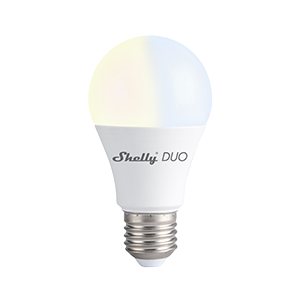
\includegraphics[scale=0.8]{images/shelly-smart.jpg}
\caption{Dispositivo Shelly.}
\label{fig:shellyduo}
\end{figure}

Nella \autoref{fig:shellyduo} si può vedere il dispositivo fisico sul quale sono stati eseguiti alcuni test che hanno confermato i risultati precedentemente ottenuti. Questa lampadina supporta la comunicazione attraverso il protocollo MQTT; infatti è possibile accenderla, spegnerla e cambiarle la luminosità e il tipo di luce da remoto. \\

La configurazione del protocollo, in questo dispositivo, avviene in una semplice interfaccia web, disponibile sulla rete al quale è connesso, in cui bisogna specificare l'indirizzo e la porta del server su cui gira il broker MQTT. È possibile anche scegliere il livello di QoS sul quale far viaggiare i pacchetti e alcuni valori come \textit{min reconnect timeout}, \textit{max reconnnect timeout} e \textit{keepalive}. Inoltre è possibile specificare username e password nel caso in cui la connessione richieda l'autenticazione dell'utente. Infine permette di specificare la flag della \textit{cleanSession} e del \textit{retain}. \\

\newcommand{\deviceshelly}{D0CC77}
Questo dispositivo mette a disposizione dell'utente diversi topic con cui lavorare; ecco quelli più importanti:

\begin{itemize}
\item \textit{shellies/announce}: in questo topic viene pubblicato un messaggio dal dispositivo che contiene informazioni utili come: \textit{id}, \textit{model}, indirizzo mac, indirizzo ip, \textit{new\_fw} e \textit{fw\_ver}. Gli ultimi due valori si riferiscono al firmware del dispositivo, il primo è una variabile booleana la quale indica se c'è un aggiornamento da eseguire, il secondo indica la versione del \textit{firmware};
\item \textit{shellies/ShellyBulbDuo-\deviceshelly/info}: fornisce alcune informazioni del dispositivo come ad esempio la rete al quale è connesso, lo stato della memoria e aggiornamenti firmware;
\item \textit{shellies/ShellyBulbDuo-\deviceshelly/light/0/command}: permette di accendere o spegnere il dispositivo passando come payload "on" o "off";
\item \textit{shellies/ShellyBulbDuo-\deviceshelly/light/0/set}: permette di modificare lo stato del dispositivo passando semplicemente un payload \textit{json};
\item \textit{shellies/ShellyBulbDuo-\deviceshelly/light/0/status}: riporta le informazioni dello stato attuale del dispositivo.
\end{itemize}

Il server broker scelto per far collegare il dispositivo è \textit{Mosquitto}. Dai test effettuati, si è visto che il dispositivo, di per sé, non ha un "anti-flood" per quanto riguarda i pacchetti ricevuti; infatti, teoricamente, è possibile, ad esempio, spegnere ed accendere la lampadina in maniera ripetuta e veloce attraverso l'invio di un publish sul topic specifico. \\

Interessanti sono stati i risultati dei test precedentemente effettuati sul broker. Ad esempio, il test nella sezione \ref{chap:publishqos2e1} è stato eseguito di nuovo, ma questa volta sul dispositivo stesso. \\
Il contenuto del file di test, ovviamente, è leggermente diverso da quello presente in \ref{chap:publishqos2e1}; in questo caso pubblichiamo due pacchetti publish dove l'unica differenza è il parametro \textit{turn}, che sul primo è "on" mentre sul secondo "off". \\

\newpage
\begin{python}
[   
    {
        "type": "publish",
        "params": {
            "topic": "shellies/ShellyBulbDuo-D0CC77/light/0/set",
            "message": "{\"brightness\":50,\"white\":50,\"temp\":2700,\"turn\":\"on\"}",
            "qos": 1,
            "dup": false,
            "retain": false,
            "packetId": 1
        }
    },
    {
        "type": "publish",
        "params": {
            "topic": "shellies/ShellyBulbDuo-D0CC77/light/0/set",
            "message": "{\"brightness\":50,\"white\":50,\"temp\":2700,\"turn\":\"off\"}",
            "qos": 1,
            "dup": false,
            "retain": false,
            "packetId": 1
        }
    },
    {
        "type": "pubrel",
        "params": {
            "packetId": 1
        }
    }
]
\end{python}
Come ci si poteva aspettare, viene pubblicato solamente il primo aggiornamento e quindi la lampadina non esegue il secondo comando che equivale a quello di spegnimento. \\

Sono stati effettuati anche altre tipologie di test, come un payload codificato stranamente o payload pesanti; in tutti i casi il dispositivo ignora il messaggio malformato non producendo alcun aggiornamento. \\

Una delicata parte di questi dispositivi è sicuramente il \textit{firmware}. Quest'ultimo è un programma implementato direttamente nel componente elettronico; nel caso di \textit{Shelly}, il firmware non è \textit{open source}, per cui non si hanno le sorgenti. I dispositivi IoT, per natura, non hanno grandi risorse: poca memoria e processori poco performanti; di conseguenza anche i software devono essere piuttosto leggeri e quindi potrebbero esserci falle di sicurezza. Gli attacchi basati su \textit{firmware} in IoT sono abbastanza comuni e rappresentano un bel problema che non è facile da arginare. In \cite{firmwareattack} sono descritte 5 categorie di attacchi basati su firmware:
\begin{itemize}
\item \textit{reverse engineering}: consiste nell'estrare il firmware ed analizzarlo, andando alla ricerca di possibili vulnerabilità;
\item \textit{firmware modification}: consiste nell'inserire codice malevolo all'interno del firmware;
\item \textit{obtaining access authorization}: se il dispositivo comunica con altri dispositivi, previa autenticazione, l'attaccante può attaccare anche quest'ultimi;
\item \textit{installing unauthorized firmware}: l'attaccante può installare un firmware malevolo per prendere il controllo del dispositivo e, ad esempio, farlo così partecipare ad una botnet;
\item \textit{unauthorized device}: consiste nell'utilizzare il firmware del dispositivo valido su uno non valido; possibili problemi di privacy. \\
\end{itemize}

Attraverso queste possibili vulnerabilità, l'attaccante può prendere il controllo del dispositivo e farlo partecipare a possibili attacchi. Ad esempio, una tipologia nuova di attacco, basato su MQTT, è descritto in \cite{articleSlowITe}. L'idea alla base è quella di inizializzare un alto numero di client col server fino ad arrivare alla saturazione del pool di connessioni del broker. \\

Oltre agli attacchi, ovviamente, un dispositivo vulnerabile può causare una violazione della privacy non di poco conto. Ad esempio, una volta che l'attaccante ha preso il controllo remoto di un dispositivo nella rete potrebbe effettuare un attacco di tipo \textit{man in the middle} per visualizzare il flusso dei messaggi dagli altri dispositivi collegati. In aggiunta a questo, l'attaccante potrebbe anche avere accesso a tutti i dispositivi domotici collegati in casa e, paradossalmente, potrebbe prendere il controllo di quest'ultima. \\

\end{large}

\chapter{Conclusioni}

\begin{large}
In questa relazione è stato descritto tutto il lavoro di studio durante l'attività di tirocinio. Inizialmente si sono cercate possibili vulnerabilità in MQTT stesso ma essendo un protocollo piuttosto semplice non è stato trovato alcunché. Invece, dai test effettuati sui differenti broker presi in esame, si son notate alcune anomalie e differenze nella gestione di alcuni test effettuati. In effetti non tutti i broker si son comportati secondo gli standard definiti per MQTT e questi esempi potrebbero essere un punto d'inizio per iniziare a rendere i comportamenti dei server uguali. \\
Per quanto riguarda il dispositivo fisico provato, si è visto che gestisce bene alcuni test strani, tuttavia manca, a mio parere, un controllo sul numero di pacchetti ricevuti in un intervallo di tempo. Nel corso della relazione si è visto come il dispositivo confermasse alcuni i test eseguiti sul broker \textit{mosquitto}. 
Nella realtà MQTT è utilizzato anche per connettere milioni di automobili fra di loro; in casi come questo è molto importante consegnare tutti i pacchetti che sono inviati. Tuttavia è possibile che ci siano due pacchetti, in un intervallo di tempo limitato, con lo stesso \textit{packet id} ma con QoS differente e così potrebbe presentarsi uno degli scenari descritti nella relazione. Il protocollo è utilizzato anche in sistemi telemetrici dove la ricezione di ogni pacchetto può essere di vitale importanza per il software.\\

Come visto nell'introduzione, il protocollo sta prendendo sempre più piede nelle piccole realtà; questo può preoccupare. Molti broker presenti in rete, infatti, non hanno alcuna protezione per l'accesso e, perciò, ci si può connettere senza problemi e rimanere in ascolto su quei canali. Inoltre, molti di questi non sono neppure aggiornati all'ultima versione di MQTT dato che utilizzano la versione 3.1.1. \\


Dopo l'attività di tirocinio sono convinto che il protocollo prenderà sempre più largo nella quotidianità anche se il tema sicurezza deve essere ancora ulteriormente approfondito. Il codice sviluppato durante il tirocinio è disponibile su GitHub \footnote{https://github.com/aedoardo/mqtt repository GitHub del progetto}.
\end{large}

\chapter*{Ringraziamenti}
\addcontentsline{toc}{chapter}{Ringraziamenti}
\begin{large}
Vorrei ringraziare, prima di tutto, il relatore della tesi \textbf{Prof. Angelo Spognardi} e il \textbf{Dr. Enrico Bassetti} per la disponibilità e per i consigli forniti durante l'attività di tirocinio. \\

Un ringraziamento anche a tutti i colleghi, diventati amici, che hanno condiviso con me questo percorso. \\

Infine ringrazio la mia famiglia per avermi aiutato a compiere questo importante passo e per essermi stata sempre vicina supportandomi in qualsiasi momento.
\end{large}

% bibliography
%\cleardoublepage
%\phantomsection
\bibliographystyle{sapthesis} % BibTeX style
\bibliography{bibliography} % BibTeX database without .bib extension

\end{document}
